%% Use this line for the final version of your report
\documentclass[final,UKenglish]{include/RaM/RaM-MScReport}

%% Use this line for the draft versions of your report, it enables rro/notes/line numbers/date in footer
%\documentclass[lineno,UKenglish]{include/RaM/RaM-MScReport}

\settitle{Development of a myocardial perfusion phantom}
\setauthor{G.J. de Vries, s1854526}
%-------------------------------------------------------------------------------------------------
% This settings.tex contains settings required for *all* documents (reports, presentations, etc)
% Project or Report specific settings should go to their own settings files (eg CE/settings.tex)
% This file is included after the class definition and before project and report specific settings 
%-------------------------------------------------------------------------------------------------

%--------Useful packages (required by the example files, turn off if you do not use them)-------
\usepackage{babel}					% Add language specific support
%\usepackage{makeidx}				% Index support
%\usepackage[totoc,justific=RaggedRight]{idxlayout}	% Make last page of index balanced and add index to toc
\usepackage{caption}				% Provides means to style captions
%\usepackage{subcaption}				% Provides support for (sub)figures and (sub)tables
%\usepackage{float}					% Improved interface for floating objects (eg figures, tables, ...)
\usepackage{enumitem}				% Add styling support to (enumerate) environments
\usepackage{listings}				% Allows (external) source files to be shown in a syntax highlighted way
%\usepackage{amsmath}				% Provides miscellaneous enhancements for documents containing formulas
\usepackage{datetime}				% Provides commands for displaying the current time
%\usepackage{etoolbox}				% Provides \AtBeginEnvironment command
\usepackage{eurosym}				% Defines \euro command to display euro symbols
%\usepackage{appendix}				% Makes it possible to modify appendix numbering
%\usepackage{longtable}				% Allows tables to span multiple pages
%\usepackage{units}					% Shows units (eg m/s) in a nice way
%\usepackage{ctable}				% Provides \ctable command for the typesetting of table and figure floats
%\usepackage{ccaption}				% Support continuation captions (eg multi-page tables)
%\usepackage{verbatim}				% Adds verbatim environment, in which texts are exactly copied to the output
%\usepackage{pdfpages}				% Include PDF pages/documents in the current document
\usepackage{color, colortbl}
\definecolor{Gray}{gray}{0.9}

\usepackage{tabularx}

\usepackage{xfrac}

\usepackage{pdflscape}

\usepackage{multicol}

%%%%%%%%%%%%%%%%%%%%%%%%%%%%%%%%%%%%%%%%%
%%%%%%% Acronyms %%%%%%%%%%%%%%%%%%%%%%%%
\usepackage{acro}

%\DeclareInstance{acro-title}{empty}{sectioning}{name-format =}

\DeclareAcronym{CT}{
	short 	= CT,
	long 	= Computed Tomography,
	class 	= abbrev
}

\DeclareAcronym{MRI}{
	short	= MRI,
	long	= Magnetic Resonance Imaging,
	alt		= MR,
	class 	= abbrev
}

\DeclareAcronym{SPECT}{
	short	= SPECT,
	long	= Single-Photon Emission Computed Tomography,
	class	= abbrev
}

\DeclareAcronym{PET}{
	short 	= PET,
	long	= Positron Emission Tomography,
	class	= abbrev
}

\DeclareAcronym{MPI}{
	short	= MPI,
	long	= Myocardial Perfusion Imaging,
	class	= abbrev
}

\DeclareAcronym{PET-MR}{
	short	= PET-MR,
	long	= PET-Magnetic Resonance,
	class	= abbrev
}

\DeclareAcronym{AIF}{
	short	= AIF,
	long	= Arterial Input Function,
	class	= abbrev
}

\DeclareAcronym{CZT}{
	short	= CZT,
	long	= Cadmium Zinc Telluride,
	class	= abbrev
}

\DeclareAcronym{CAD}{
	short	= CAD,
	long	= Coronary Artery Disease,
	class	= abbrev
}

\DeclareAcronym{VC} {
	short	= VC,
	long	= Vena Cava,
	class	= abbrev
}

\DeclareAcronym{PA}{
	short				= PA,
	long				= Pulmonary Artery,
	long-plural-form 	= Pulmonary Arteries,
	short-plural		= s,
	class	= abbrev
}

\DeclareAcronym{PV}{
	short				= PV,
	long				= Pulmonary Vein,
	long-plural 		= s,
	short-plural		= s,
	class	= abbrev
}

\DeclareAcronym{PMT}{
	short			= PMT,
	short-plural	= s,
	long			= Photomultiplier Tube,
	long-plural		= s,
	class			= abbrev
}
%%%%%%%%%%%%%%%%%%%%%%%%%%%%%%%%%%%%%%%%%%%%%%%%
%%%%%%%%%%%%%%%% END ACRONYM %%%%%%%%%%%%%%%%%%%

\usepackage{include/files/requirements}

\iffinalversion
	\usepackage[final]{include/files/notes}% Add note commands, [final] removes all notes from the document
	\usepackage[final]{include/files/rro}  % Add Rich Report Outline support, [final] removes all RRO output from document
\else
	\usepackage{include/files/notes}       % Add note commands
	\usepackage{include/files/rro}         % Add Rich Report Outline support
\fi

% Add wrongly (or unknown) hyphened words here (space separated and - at possible hyphenation positions):
%\hyphenation{}

%% Spacing possibilities for captions are available as well
% See captions.pdf for all options!
\captionsetup{font=small,labelfont=bf}

%% Center all figures by default
%% http://tex.stackexchange.com/questions/2651/should-i-use-center-or-centering-for-figures-and-tables
\makeatletter
\g@addto@macro\@floatboxreset\centering
\makeatother

%% Make use small font size in verbatim environment
% Note: AtBeginEnvironment is provided by etoolbox package
%\AtBeginEnvironment{verbatim}{\small}

%% Include verbatim in the subfigure env
% From: subfig.pdf, section 4.4
% <Uncomment if verbatim is required in subfloat>:
%\makeatletter
%\newbox\sf@box
%\let\orig@subfloat\subfloat
%\renewenvironment{subfloat}[2][]%
%{ \def\sf@one{#1}%
%  \def\sf@two{#2}%
%  \setbox\sf@box\hbox
%  \bgroup}%
%{ \egroup
%  \ifx\@empty\sf@two\@empty\relax
%    \def\sf@two{\@empty}
%  \fi
%  \ifx\@empty\sf@one\@empty\relax
%    \orig@subfloat[\sf@two]{\box\sf@box}%
%  \else
%    \orig@subfloat[\sf@one][\sf@two]{\box\sf@box}%
%  \fi}
%\makeatother
%% Uncomment till here
  
%% Automatically provide H option for floats
% Requires float package
% \floatplacement{figure}{H} 
% \floatplacement{table}{H} 

%% abbreviation making
\newcommand{\abbr}[1]{(\textit{#1})}

%%lstlisting settings
\lstset{	%aboveskip=20pt,%
		numbers=none, %no line numbers
%		numbers=left, %show line numbers
		numberstyle=\tiny,%
		frame=single,%
		frameround={t}{t}{t}{t},%
		numbersep=5pt,%
%		language=C,% (default) code language in the document
		captionpos=b,%
		xleftmargin=2em,
		framexleftmargin=1.5em,
		xrightmargin=2em,
		framexrightmargin=1.5em,
		morecomment=[s][\itshape]{<}{>}, %also define <> as comment
		morecomment=[s][\itshape]{[}{]} %also define [] as comment
}

%lstinline with empty language definition
\lstdefinelanguage{empty}{}
\newcommand{\mylstinline}[1]{{\lstinline[language=empty]{#1}}}

% Default value of top separator (empty space) of lists
\setlist{topsep=4pt}

%% Don't show warnings like: ``PDF inclusion: found PDF version <1.x>, but at most version <1.4> allowed
% Uncomment if you experience these kind of warnings 
%\ifpdf
%	\pdfminorversion=6 
%\fi


\begin{document}
% Numbered roman style

\makerro				% Build RichReportOutline.rro file

\frontmatter


\includepdf{./frontpage/frontpage_r1d0.pdf}

% Use \maketitle or the available PDF when it is released (for student reports)
\maketitle

% Enter the name of the official RaM title page PDF between the brackets
% ! This method disables the option of using EPS files in your report.
% ! If EPS images are required, use LaTeX source instead of the PDF file
% 
\includepdf{./frontpage/frontpage_r0d1.pdf}
\cleardoublepage

% \include{Summary}
% Dutch summary is not obligatory
%\include{Samenvatting}

\chapter*{Preface}

\vskip-10pt
The system requirements specify all the requirements for the myocardial perfusion phantom. These requirements are based on research and interviews with stakeholders.

\vskip50pt
G.J. (Gijs) de Vries\\
Enschede, 7\textsuperscript{th} of January 2019
%In a two-sided printing style, it makes the next page a right-hand
% (odd-numbered) page, producing a blank page if necessary.
\cleardoublepage

% Add the table of contents pages (TOC)
\tableofcontents

% The report starts here
\mainmatter

% this contains a showcase of LaTeX
\chapter{Introduction}
\label{ch:Intro}

\rrod{Read into background information on D-SPECT}
\rrod{Write global background information}
\rrod{Introduce the rest of the document}
\rrod{Assignment was for dynamic SPECT scanning, but is that the same as using the D-SPECT? The D-SPECT can scan dynamically, and is available in ZGT}
\rrod{Too much SPECT detail in introduction? Moved to literature}
\rrot{Give arguments why to choose SPECT}

\Ac{MPI}, or, simply put, the imaging of the blood flow in the heart muscle, plays an important role in diagnosing heart failure or detecting \ac{CAD}. Imaging systems like \ac{CT}, \ac{MRI}, \ac{SPECT}, or \ac{PET} can visualise a (radioactive) contrast bolus in the supplying arteries and in underlying myocardial tissue, whose flow can give an indication of narrowed or blocked blood vessels.

Many variations in the visualisation process of myocardial perfusion, including variations in hard- and software, can (significantly) influence the outcome and in turn have consequences for patient treatment. These variations need to be validated against a well-known baseline.

The goal of the project is to develop a prototype myocardial perfusion phantom capable of repeated simulations of typical and cardiac defect situations using clinical software commonly used in myocardial perfusion scans. Most software packages require anatomical recognition points which imposes anatomical requirements on the phantom. In addition, the phantom can be used for educational and training purposes to demonstrate the impact of (poorly) chosen variables, e.g. pressure or flow, scanning parameters, cardiac defects, and so forth.

\section*{Document overview}
\label{sec:doc_overview}
\rrod{Update in correspondence with meeting december 10}
The project plan consists of a literature review of existing myocardial perfusion phantoms, their comparison to human physiology, and a discussion between the different types of scanners. The literature is followed by the research methodology containing the research questions and goals of the project. The detailed planning is the last section of the project plan stating workdays and -weeks, off-days, deadlines, and meetings.

\section*{Abbreviations}
\begin{multicols}{2}
	\printacronyms[include-classes=abbrev, name=Abbreviations, heading=none]
\end{multicols}

% add another chapter
% change file name for better descriptive names, but start with ch-
\chapter{Literature}
\label{ch:literature}
\rrow{Read available literature}
\rrow{Write literature review to more accurately define research questions}
\rrow{D-SPECT literature?}
\rrot{Discuss division of work}
\rroi{Dialysis tube mimics capillaries and not tissue?}
\rroi{Mathys reported that no literature was found that manufacturers calibrate their scanners.}

\section{Phantoms}
\subsection{Magnetic Resonance}
\rrow{Shift the limitations to later section}
\cite{noguchi2007quantitative} developed a simple phantom that consists of a syringe, diameter of 40mm, beads, and tubes, diameter of 4mm. The perfusate, 0.1mM GD-DTPA doped 8L water solution, flows through the beads, to disturb the flow, and then perfuses through parallel tubes, to prevent cross-current. The perfusate is tagged at the beads while the images are taken at 5 parallel planes, perpendicular to the tubes. The actual measured flow is the average obtained from the parallel planes. 

\cite{ebrahimi2010microfabricated} created a phantom using microfabrication to create a microvasculature on 4-inch ($\approx$ 10cm) silicone wafers. The microvasculature is build up from four blocks, containing 4x2 (RxC) cells. Each cell is build up from 100 "features" separated by 25$\mu$m tracks. These tracks provide many different paths for perfusate to flow, effectively simulating capillaries in tissue. A $300\mu L$ bolus of a distilled water solution containing 25mM/L of Manganese.

\cite{wang2010flow} used a heamodialysis filter connected to a nonpulsatile pump. A static water phantom was placed next to the haemodialysis filter to show that it cancels out between tag (with magnetic labelling) and control (no magnetic labelling) images.

\cite{anderson2011semipermeable} extracted hollow fibres from haemodialysis filters to create their own single-fibre and multi-fibre phantom. Similar to some standard haemodialysis filters, their phantoms have access to both the extracellular space (i.e. the fluid outside of the fibres) and intracellular space (i.e. the fluid inside the fibres). As the name suggests, their single-fibre phantom consists of an individual fibre placed inside a capillary tube. The multi-fibre phantom consists of a variable amount of fibres that are placed in a heat-shrink tube. A four-way valve switched between the main perfusate and a aquesous solution of 0.2 mM GD-BOPTA.

\cite{chiribiri2013perfusion} developed a four chambered anatomic phantom that resembles the heart of a 60kg person. The four chambers correspond to the four chambers of the heart, sized to match the physiological size. In addition, a \ac{VC}, \ac{PA}/\ac{PV} combination, and an aorta are present in the phantom. Contrast is injected in the same manner as is performed in patients; in a vein. In the phantom, the contrast is injected directly into the vena cava via a three-way stopcock. The contrast moves through the phantom's right atrium, right ventricle then via the \ac{PA}/\ac{PV} to the left chamber and finally to the left ventricle. The phantom is not capable of simulating the contrast's behaviour in the lungs since the \ac{PA} is directly connected to the \ac{PV}. Two myocardial chambers (one active and one control), the \ac{VC}, \ac{PA}, \ac{PV} and the aorta are in the imaging plane where the proximal part of the aorta, where the aorta branches to the myocardium, is used for the \ac{AIF}. 

\cite{otton2013direct} used the same phantom to compare \ac{CT} against \ac{MRI}. In addition to the previous authors, \cite{o2017effect} used a water-filled torso phantom to ensure more anatomically correct image in \ac{PET-MR}.

\subsection{Computed Tomography}
\cite{teslow1991x} developed a cylindrical perfusion phantom, shaped like the left ventricle of a dog. It has a 6.5cm outer diameter, 4.5cm inner diameter, and a length of 6.5cm. The authors specifically used methyl methacrylate plastic since it gives similar radiographic image as tissue and blood. Additionally, a solid plastic cylinder, placed in the centre, is used to attenuate x-ray beams similar to the attenuation of a blood-filled dog's ventricle. The capillaries are simulates by means of different sized nylon balls of 0.318, 0.476, and 0.635cm. The smallest balls are packed near the outlet, while the medium sized balls are packed at the inlet, and the largest balls are placed in between. The authors do not go into detail on the used contrast agent, other than  10ml of a radio-opaque indicator is injected for one second.

\cite{klotz1999perfusion}

\cite{driscoll2011development} developed a 10cm long, with a diameter of 5cm, phantom with two inputs, only one is used, and two outputs. The capillaries are simulated by means of a vinyl tube where mass can be exchanged with the main cylinder via sets of small holes on either side of the cylinder. The output of the vinyl tube and the output of the shell combine, and feeds back through the imaging area to validate outward going flow, which should be the same as the input flow. Their \ac{AIF}, however, is created by means of a programmable pump which injects in the form of a typical clinical \ac{AIF} rather than having a system-based \ac{AIF}. The Visipaque\textsuperscript{TM} (iodixanol) 270 mgI/ml is injected into a blood-mimicking fluid consisting of 40\% glycerol and 60\% water.

\cite{ganguly2012vitro} developed an interestingly, slightly different phantom than other;  a linearly moving phantom. The phantom itself is a cylinder, 1.9cm inner diameter, with a length of 32.2cm. It contained 64 different compartments of 0.5cm in height separated by a 0.5mm thick carbon fibre wall. Every compartment had a single opening where contrast, 300mgI/Omnipaque, is injected. The concentration of contrast that is injected in subsequent compartments, resemble a sinusoidal signal. This phantom is placed on a linear motor which moves the phantom parallel to the patient's bed. The author's goal is to compare and determine the temporal accuracy of the imaging system. To simulate the attenuation of the head, a 15cm cylindrical, water-filled, phantom was placed around the perfusion phantom. 

\cite{mathys2012phantom} developed a similar phantom that consists of two cylinders, a smaller (4cm diameter) inside a larger (11cm diameter) cylinder. Water flows via four tubes into the inner cylinder where it flows outward into the larger cylinder that contains 1.5mm polyoxymethylene globes as tissue replacement. The larger cylinder is drained by four holes. 2mL of contrast, Accupaque 300, is injected followed by 15 of saline at 5mL/s using a double-head injector.

\cite{boese2013performance} developed a cylindrical phantom for brain perfusion measurements in a C-arm. Their phantom utilises a combination of large arteries, smaller arteries, and a sinter board for the capillaries. The main artery splits into smaller arteries which in turn splits into sixteen even smaller ones that connect to the sinter board. The upper two arteries have an inner diameter of 1.7mm representing the carotid arteries and the lower two arteries have an inner diameter of 1.0mm representing vertebral arteries. The authors used a very specific contrast injection protocol: relatively large pre-injection of 21mL NaCl, followed by a variable amount of Imeron 400, and ended by a 6mL post-injection of NaCl, all at 6mL/s.

\cite{suzuki2017quantitative} designed a straight-forward \ac{CT} phantom that uses a dry-type haemodialyser with a pressurised dialysate space to prevent the perfusate from leaving the hollow fibres. The authors varied the dose in order determine the effects on the perfusion indices. They maintained a constant volumetric flow, Q, and concluded that the perfusion indices are susceptible to dose conditions. 

\cite{hashimoto2018effect} used the same phantom in combination with a commercially synthetic bone layer such that quantification software recognises the phantom as a human head. Instead of varying the dose, the contrast injection protocol and the scanning interval are varied based on their hypothesis that it would increase the quantitative accuracy. However, they concluded that they are independent factors when using the b-SVD algorithm. 

\subsection{Ultrasound}
\rrod{Veltmann phantom}

\cite{veltmann2002design} designed a flow phantom that consists of a high- and low flow circuit. The high flow circuit consists of a \textit{heated} reservoir flowing into a haemodialysis cartridge, which filters any residue micro-bubbles (contrast agent) and removes air bubbles, before entering a second haemodialysis cartridge, the perfusion cartridge. Perfusate that does not enter the capillaries is returned to the reservoir passing a variable resistance. The perfusate that does enter the capillaries of the perfusion cartridge, is controlled by a gear pump, which simultaneously acts as a variable flow resistance for the low flow circuit. After the gear pump, a third haemodialysis filter filters the microbubbles from the perfusate. The authors performed two different experiments, one with an unmodified haemodialysis filter and one with a haemodialysis filter that has the majority of the lower capillaries glued shut. The contrast agent tends to float, especially in the low flow circuit. By decreasing the number of perfused capillaries, the flow is made more homogeneous and avoids attenuation in the lower areas. Both \cite{sakano2015power} and \cite{lohmaier2004vitro} use this phantom setup.

\cite{kim2016efficiency} performs perfusion experiments using ultrasound without adding any contrast. Similar to the \ac{CT} and \aca{MRI} phantoms, a dialysis tube is used to mimic human capillaries. The dialysis tube is submerged in water and part of the plastic case was removed, replaced by a latex foil as proposed by \cite{veltmann2002design}, such that it creates an acoustic window. More interestingly, \cite{kim2016efficiency} use a secondary, 1Hz, peristaltic pump to simulate cardiac motion. \cite{gauthier2011perfusion} uses a peristaltic pump after a renal dialysis cartridge to create a pulsatile, but constant, flow. They do not use a secondary pump for the extracellular space.

\subsection{Positron Emission Tomography / Single-Photon Emission Computed Tomography}
Although the phantoms are not specifically designed for \ac{PET} or \ac{SPECT} scanning, the previously mentioned phantoms can be an inpsirational source for \ac{PET}/\ac{SPECT} phantoms. The different technology requires a new approach to some (or many) of the materials used.

\subsection{Phantom discussion}
The phantom by \cite{chiribiri2013perfusion} is unable to simulate the diffusion of contrast into heart tissue or the interstitial space, as admitted by the authors and confirmed by \cite{otton2013direct, o2017effect}. Furthermore, \cite{chiribiri2013perfusion} mentioned that the blood flow resistance is lower than in patients due to its complexity.

The findings of \cite{otton2013direct} are similar; the contrast curves represent those obtained from clinical trials and since the phantom can be used in a clinical \aca{MRI} scanner, the gap between phantom and clinical studies is decreased. Even with the addition of a water-filled torso phantom, it is still unable to mimic respiratory or cardiac motion \citep{o2017feasibility}.

\rroi{Is contrast absorbed by tissue in the brain? Read something about the blood-brain barrier preventing such things.}
The straight forward phantom of \cite{suzuki2017quantitative} does not resemble the human brain, which caused problems in certain programs, and the capillary possessions is much greater than in clinical situations. This may ultimately compromise the reliability of the phantom to mimic clinical situations. Although \cite{hashimoto2018effect} uses a commercially synthethic bone layer, the phantom does not simulate contrast uptake by surrounding tissue which does occur in myocardial perfusion measurements.
\section{Physiology}


\section{Technology}
\subsection{SPECT}
The imaging method in a typical \ac{SPECT} scanner are scintillator-based gamma cameras, also known as Anger cameras. Gamma cameras use a scintillator to "transduce" gamma radiation, originating from an injected tracer, to photons. Part of these photons are directed towards a photocathode. If a quantum of light hits the photocathode, which is coated with a photosensitive coating, electrons are emitted due to the photoelectric effect. These electrons travel through a \acp{PMT} and hitting series of dynodes, which in turn trigger secondary emission effectively multiplying the number of electrons travelling through the tube. Electrons hitting the last dynode, which is known as the anode, cause a current pulse which can be detected by measuring equipment. It is proportional to the amount of gamma ray photons entering the scintillator\citep{CZTTech2009}.

\subsection{Digital SPECT}
Developments in imaging systems gave rise to the digital \ac{SPECT} scanner. In contrast to the analogue Anger cameras, the digital \ac{SPECT} scanner utilises a direct conversion semiconductor: \ac{CZT}. \cite{wagenaar2004cdte} used \ac{CZT} to develop pixelated detector units which could then be used for medical imaging. In a recent study, it is shown that a digital \ac{SPECT} scanner, using multiple pixelated \ac{CZT} detectors, showed significant improvements in image sharpness and contrast\citep{goshen2018feasibility}. These detector units do not require any \acp{PMT} and thus allow for a more compact and flexible design \citep{erlandsson2009performance}. The D-SPECT scanner, a digital \ac{SPECT} scanner developed by Spectrum Dynamics\footnote{https://www.spectrum-dynamics.com/}, offers improvements in sensitivity and energy resolution \citep{SpectDynam2018} over Anger camera systems. However, these digital systems are relatively new and require proper validation to convince medical personnel of its value.

\subsection{Scanner comparison}
As is previously mentioned, there are various types of scanners that use different techniques, \ac{CT} \ac{MRI}, or Scintigraphy based (\ac{SPECT}/\ac{PET}) scanners. In cardiology, the \ac{SPECT} scanner is widely employed for coronary and myocardial perfusion measurements \citep{rahmim2008pet}. It is known that \ac{PET} scans are generally more expensive \citep{hlatky2014economic, RadioPead2018}. \cite{hlatky2014economic} followed patients for two years, recording the costs and concluded that \ac{PET} costs are 22\% higher than the costs for \ac{SPECT} for patients with suspected \ac{CAD}.
\chapter{Research methodology}
\label{ch:res_metho}
\rrod{Define research questions}
\rrod{Discuss main research question}
\rrot{Define research boundaries}
\rrod{Define project goals}
\rrod{Implement scanner descision, became research question, will be answered in SR.}
\rrod{Use limitations of phantoms to lead to research question}

Different perfusion phantoms have been developed. Some are specifically designed to simulate the myocardial perfusion \footnote{\citep{chiribiri2013perfusion, otton2013direct, o2017effect, o2017feasibility, teslow1991x}}, others for brain perfusion \footnote{\citep{hashimoto2018effect, suzuki2017quantitative, boese2013performance, mathys2012phantom, ebrahimi2010microfabricated, wang2010flow, noguchi2007quantitative, ganguly2012vitro, klotz1999perfusion}}, or capillaries in general \footnote{\citep{kim2016efficiency, anderson2011semipermeable, driscoll2011development, gauthier2011perfusion, veltmann2002design, lohmaier2004vitro}}, and even phantoms to simulate perfusion in rheumatoid finger joints \citep{sakano2015power} and skin \citep{kim2018multidimensional}. Most software packages are designed for human organs and look for landmarks such that it can perform the most optimal calculation. Many of these phantoms do not resemble human anatomy. The phantom proposed by \cite{chiribiri2013perfusion}, the four-chambered heart, comes close to mimicking a human heart. However, the myocardium chamber is simplified and not covering the chambers. Furthermore, the phantoms are unable to mimic cardiac defects. These anatomical anomalies, and the inability to mimic cardiac defects,  results in the need for a new phantom.

\section{Research questions}
\begin{figure}[b!]
	\begin{center}
		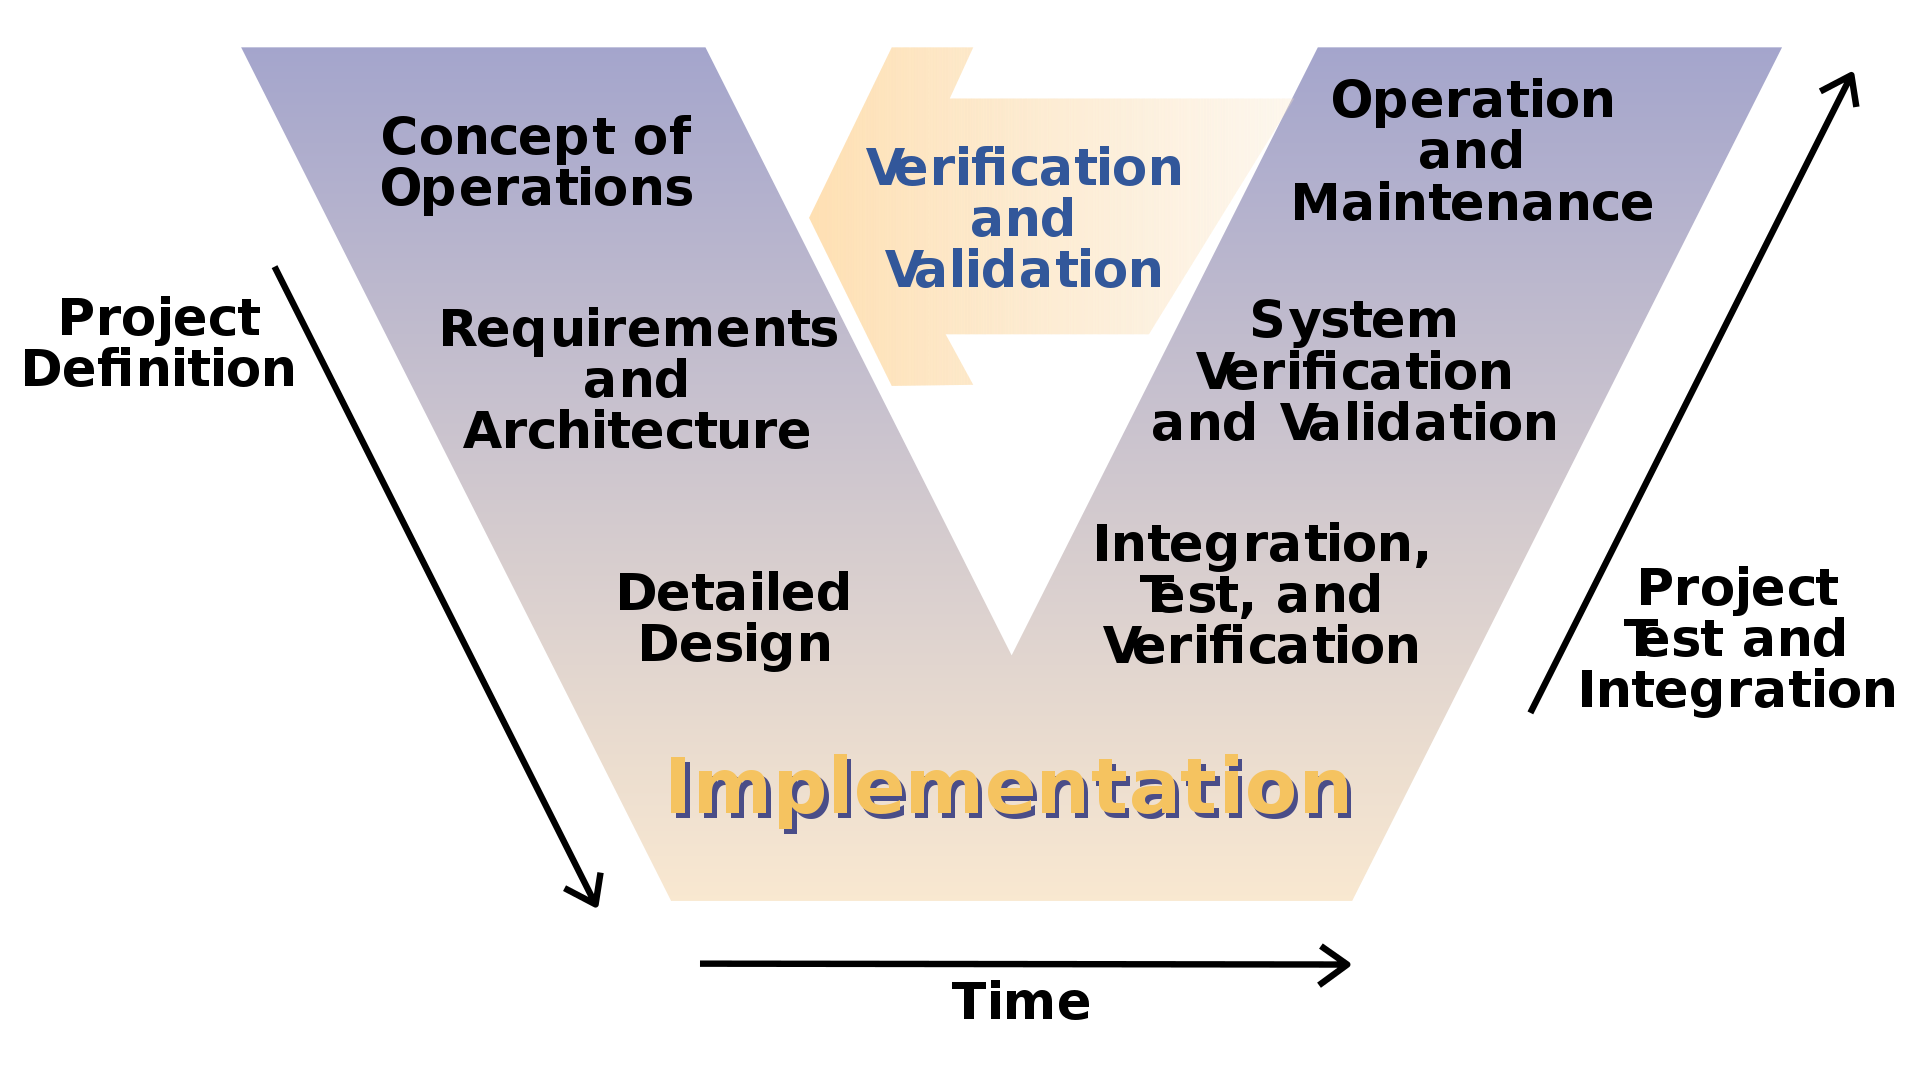
\includegraphics[width=0.5\linewidth]{images/vmodel.png}
	\end{center}
	\caption{V-Model\citep{rook1986controlling} as proposed by \cite{osborne2005clarus}}
	\label{fig:vmodel}
\end{figure}

The project is carried out using the V-Model \citep{rook1986controlling,osborne2005clarus} approach, see figure \ref{fig:vmodel}. The research questions are defined based on the project definition phase.

\subsection{Concept of operations}
Which type (CT, MRI, PET, or SPECT) of scanner should be used for myocardial perfusion imaging based on technology and availability?

What must the myocardial perfusion phantom be able to simulate?

\subsection{Requirements and Architecture}
What are the requirements for a myocardial perfusion phantom that can be used in combination with commonly used clinical software?

\subsection{Detailed Design}
How can the myocardial perfusion phantom meet the clinical requirements and mimic the perfusion of a human heart?

\section{Project goal}
The goal of the project is to develop a prototype myocardial perfusion phantom capable of reproducible simulations of typical and cardiac defect situations using clinical software commonly used in myocardial perfusion scans. Most software packages require anatomical landmarks which imposes requirements on the phantom. In addition, the phantom can be used for educational and training purposes to demonstrate the impact of (poorly) chosen variables, e.g. pressure or flow, scanning parameters, cardiac defects, and so forth.

\subsection*{Project sub-goal}
During the individual project, a calibration set-up for flow and pressure sensors has been developed. The prototype version showed that flow sensors can be calibrated using the "emptying tank" principle. Pressure sensors have not been implemented in the prototype. Furthermore, the calibration set-up relies too much on human interaction. A sub-goal of the project will be to improve the existing calibration set-up such that flow and pressure sensors can be calibrated which in turn will increase the reliability of the flow set-up.

\section{Stakeholders}
\label{sec:stakeholders}
A distinction is made between direct stakeholders, actively involved in the development, indirect stakeholders, can provide knowledge or resources, and beneficial stakeholders, (potentially) benefit from the development.

\begin{tabular}{lll}
 	\multicolumn{1}{c}{\textbf{Direct}} & \multicolumn{1}{c}{\textbf{Indirect}} & \multicolumn{1}{c}{\textbf{Beneficial}} \\
	 - C.H. (Kees) Slump, &  - Marcel Greuter, & - Patients with suspected \ac{CAD}, \\
	 - M.E. (Marije) Kamphuis, & - Riemer Slart, & - Scanner manufacturers,\\
	 - Clinical Physicists, & - Willem van Meurs. & - Scanner software developers, \\
	 - Lab technicians, & & - Hospitals. \\
	 - Nuclear Medicine Physicians, & & \\
	 - Cardiologists. & & \\
\end{tabular}

\section{Approach}
The research questions will primarily be answered by means of literature and by interviews with the stakeholders, see section \ref{sec:stakeholders}. They are regularly involved with myocardial perfusion imaging and are thus familiar with the clinical software, hardware, work flow, and requirements. These interviews will provide additional (practical) insight.

Part of the V-Model approach is the continuous feedback. Requirements and designs are constantly updated according to new insights acquired during the development process. 

\subsection{General concept}
\begin{figure}[b!]
	\begin{center}
		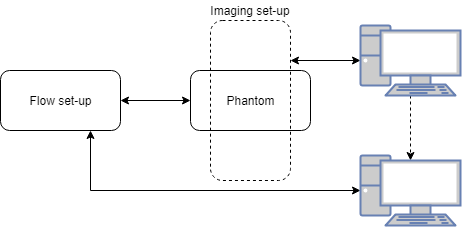
\includegraphics[width=0.75\linewidth]{images/global_setup.png}
	\end{center}
	\caption{General concept, schematic}
	\label{fig:general_concept}
\end{figure}
A general concept is shown in figure \ref{fig:general_concept}. Three main parts can be identified: flow set-up, phantom, and imaging device. The flow set-up consists of everything to produce and maintain pressures and/or flows and measure these variables. The user-interface is a computer or laptop. The phantom consist of everything needed to mimic cardiac defects and to provide a representative image for myocardial perfusion image processing software. The imaging set-up consists of the imaging device itself along with any contrast agents needed to properly image the phantom. Many imaging devices communicate with a dedicated workstation on which the image processing software runs.

\section{Boundaries}
The project is carried out as an Electrical Engineering's final thesis project of 40 \ac{ECTS}. The boundaries for the project is to design and build a flow phantom capable of simulating myocardial blood flow according to specified, and agreed upon, system requirements. These system requirements require research, interviews and knowledge on physiology and are thus part of the project. The phantom and its set-up are part of research performed by M.E. (Marije) Kamphuis and imposes additional requirements on the project. The project is a tool for Marije to answer her research questions, but answering these research questions is not part of the final thesis. 

\section{Additional resources}
During the individual project of G.J. (Gijs) de Vries, a prototype flow set-up, control module, and calibration set-up has been realised and can be used / re-cycled.
\subsection{Flow set-up}
The flow set-up uses simple, low costs pumps and available flow sensors. These might not be suitable for high precision flow systems. It is encouraged to look into alternatives.
\subsection{Control module}
The control module requires improvement when it is to be re-used. Two of the main improvements consist of improving the electro(magnetic) shielding to decrease the susceptibility to noise and to optimise the pump controllers.

\chapter{Planning}
\label{ch:Planning}
\rrot{Create graphical planning}
\rrot{Create workday overview}
\rrot{Create week overview}
\rrot{Define deadlines}
\rrot{Define meetings: frequency, type, and already planned}


% Appendix starts here
% change file name for better descriptive names, but start with apx-
\appendix
\chapter{Appendix 1} \label{app:one}

\chapter{Appendix: Normal heart rate/blood pressure and myocardial perfusion rates by Ho et al. (2014)}\label{app:physoverview_ho}
The following tables summarise \cite{ho2014dynamic}.
\begin{table}[h!]
\caption{Heart rate and blood pressure according to \cite{ho2014dynamic}.}
This table shows the heart rate and blood pressure in \citep{ho2014dynamic} among 35 patients with documented \ac{CAD} and 35 control (low-risk) patients. The 35 documented CAD patients are from a previous study.
\begin{tabular}{l|l|cc|}
          \multicolumn{1}{c}{ } & \multicolumn{1}{c}{ } &  \multicolumn{1}{c}{\textbf{Control}} & \multicolumn{1}{c}{\textbf{Stenosis}} \\
          \cline{2-4}
\multirow{2}{*}{\textbf{Heart rate} [BPM]} &  Base line &  $66\pm 10$ &  $73\pm 14$  \\
& MV* &  $88.54\pm 11.45$ & $82\pm 16$   \\
\cline{2-4}
\multirow{4}{*}{\textbf{Blood pressure} [mmHg]} & Diastolic (B) & $63\pm 13$ & $-$ \\
& Diastolic (MV)& $56 \pm 10$ & $-$ \\
& Systolic (B) 	& $111\pm 17$ & $-$ \\
& Systolic (MV) & $105\pm 21$ & $-$ \\
\cline{2-4}
\end{tabular} \\
\raggedright
\textit{* \acf{MV}}
\label{tab:ho_physfact}
\end{table}

\begin{table}[h!]
\caption{Myocardial blood flow according to \cite{ho2014dynamic}.}
This table shows the myocardial perfusion rates by \cite{ho2014dynamic}, given in mL/min/100g.\\
\begin{tabular}{l|ccc|}
			\multicolumn{1}{c}{ } & \multicolumn{1}{c}{\textbf{Low risk}} & \multicolumn{1}{c}{\textbf{Historic ischaemia}} & \multicolumn{1}{c}{\textbf{Previous infarction}} \\
          \cline{2-4}
Global rest 	& $74.08\pm 16.3$ & $82.29\pm 16.87$ & $81.98\pm 18.54$\\
Global stress   & $141.92\pm 30.83$ & $107.95\pm 25.25$ & $106.93\pm 32.91$\\
\cline{2-4}
\end{tabular} \\
\label{tab:hoFlows}
\end{table}

% Bibliography starts here
\backmatter

% Generate bibliography
\fancyhead[LO]{Bibliography}
\bibliographystyle{include/files/RaM-bibtex}
\label{ch:bib} %label to refer to
\bibliography{bibliography} 

\end{document}

